\chapter{Mathematical induction}
\begin{epigraphs}\qitem[author={George Boole}]{It is sometimes required to prove a theorem which shall be true whenever a certain quantity \(n\) which it involves shall be an integer or whole number and the method of proof is usually of the following kind. 1st. The theorem is proved to be true when \(n = 1\). 2ndly. It is proved that if the theorem is true when \(n\) is a given whole number, it will be true if \(n\) is the next greater integer. Hence the theorem is true universally.}\SubIndex{Boole, George}
\qitem[author={Jonathan Swift}, source={On Poetry: A Rhapsody}]{%
So nat'ralists observe, a flea \\
Has smaller fleas that on him prey; \\
And these have smaller fleas to bite 'em. \\
And so proceeds Ad infinitum.}\SubIndex{Swift, Jonathan}\SubIndex{flea}
\end{epigraphs}
\begin{example}
It is often believed that everyone with red\SubIndex{red hair}\SubIndex{hair!red} hair must have a red haired ancestor.
But this principle is not true.
We have all seen someone with red hair.
According to the principle, she must have a red haired ancestor.
By the same principle, he must have a red haired ancestor too, and so on.
So the principle predicts an infinite chain of red haired ancestors.
But there have only been a finite number of creatures (so the geologists tell us).
So some red haired creature had no red haired ancestor.
\end{example}
\begin{example}
We will see that 
\[
1+2+3+\dots+n = \frac{n(n+1)}{2}
\]
for any positive integer \(n\).
First, let's check that this is correct for a few values of \(n\) just to be careful.
\emph{Danger:} just to be \emph{very} careful, we put \(\equalquestion\) between any two quantities when we are \emph{checking} to see if they are equal; we are making clear that we don't yet know.

For \(n=1\), we get \(1 \equalquestion 1(1+1)/2\), which is true because the right hand side is \(1(1+1)/2)=2/2=1\).

For \(n=2\), we need to check \(1+2 \equalquestion 2(2+1)/2\).
The left hand side of the equation is \(3\), while the right hand side is:
\[
\frac{2(2+1)}{2}=\frac{2(3)}{2}=3,
\]
So we checked that they are equal.

For \(n=3\), we need to check that \(1+2+3 \equalquestion 3(3+1)/2\).
The left hand side is \(6\), and you can check that the right hand side is \(3(4)/2=6\) too.
So we checked that they are equal.

But this process will just go on for ever and we will never finish checking all values of \(n\).
We want to check \emph{all} values of \(n\), all at once.
\end{example}
Picture a row of dominoes.\SubIndex{domino}
If we can make the first domino topple, and we can make sure that each domino, if it topples, will make the next domino topple, then they will all topple.
\begin{theorem}[The Principle of Mathematical Induction\define{mathematical induction}\define{induction}]
Take a collection of positive integers.
Suppose that \(1\) belongs to this collection.
Suppose that, whenever all positive integers less than a given positive integer \(n\) belong to the collection, then so does the integer \(n\).
(For example, if \(1, 2, 3, 4, 5\) belong, then so does \(6\), and so on.)
Then the collection consists precisely of all of the positive integers.
\end{theorem}
\begin{proof}
Let \(S\) be the set of positive integers \emph{not} belonging to that collection.
If \(S\) is empty, then our collection contains all positive integers, so our theorem is correct.
But what is \(S\) is \emph{not} empty?
By the law\SubIndex{law of well ordering} of well ordering, if \(S\) is not empty, then \(S\) has a least element, say \(n\).
So \(n\) is \emph{not} in our collection.
But being the least integer not in our collection, all integers \(1, 2, \dots, n-1\) less than \(n\) \emph{are} in our collection.
By hypothesis, \(n\) is also in our collection, a contradiction to our assumption that \(S\) is not empty.
\end{proof}
\begin{example}
Let's prove that \(1+2+3+\dots+n=n(n+1)/2\) for any positive integer \(n\).
First, note that we have already checked this for \(n=1\) above.
Imagine that we have checked our equation \(1+2+3+\dots+n=n(n+1)/2\) for any positive integer \(n\) up to, but not including, some integer \(n=k\).
Now we want to check for \(n=k\) whether it is still true: \(1+2+3+\dots+n\equalquestion n(n+1)/2\).
Since we already know this for \(n=k-1\), we are allowed to write that out, without question marks:
\[
1+2+3+\dots+(k-2)+(k-1)=(k-1)(k-1+1)/2.
\]
Simplify:
\[
1+2+3+\dots+k-1=(k-1)k/2.
\]
Now add \(k\) to both sides.
The left hand side becomes
\(
1+2+3+\dots+k
\).
The right hand side becomes \((k-1)k/2+k\), which we simplify to
\begin{align*}
\frac{(k-1)k}{2} + k 
&=
\frac{(k-1)k}{2} + \frac{2k}{2},
\\
&=
\frac{k^2-k \, + \, 2k}{2},
\\
&=
\frac{k^2+k}{2},
\\
&=
\frac{k(k+1)}{2}.
\end{align*}
So we have found that, as we wanted to prove,
\[
1+2+3+\dots+k = \frac{k(k+1)}{2}.
\]
Note that we \emph{used} mathematical induction to prove this: we prove the result for \(n=1\), and then suppose that we have proven it already for all values of \(n\) up to some given value, and then show that this will ensure it is still true for the next value.
\end{example}
The general pattern of induction arguments: we start with a statement we want to prove, which contains a variable, say \(n\), representing a positive integer.
\begin{enumerate}
\item \emph{The base case:} Prove your statement directly for \(n=1\).
\item \emph{The induction hypothesis:} Assume that the statement is true for all positive integer values less than some value \(n\).
\item \emph{The induction step:} Prove that it is therefore also true for that value of \(n\).
\end{enumerate}
\begin{example}
We can use induction in definitions, not just in proofs.
We haven't made sense yet of exponents.
(Exponents are often called \emph{indices} in Irish secondary schools, but nowhere else in the world to my knowledge).
\begin{enumerate}\itemsep2pt
\item \emph{The base case:} For any integer \(a \ne 0\) we define \(a^0\defeq 1\).
\emph{Watch:} We can write \(\defeq\) instead of \(=\) to mean that this is our \emph{definition} of what \(a^0\) \emph{means}, not an equation we have somehow calculated out.
For any integer \(a\) (including the possibility of \(a=0\)) we also define \(a^1 \defeq a\).
\item \emph{The induction hypothesis:} Suppose that we have defined already what \[a^1, a^2, \dots, a^b\] means, for some positive integer \(b\).
\item \emph{The induction step:} We then define \(a^{b+1}\) to mean \(a^{b+1} \defeq a \cdot a^b\).
\end{enumerate}
For example, by writing out
\begin{align*}
a^4 
&=
a \cdot a^3,
\\
&=
a \cdot a \cdot a^2,
\\
&=
a \cdot a \cdot a \cdot a^1,
\\
&=
\underbrace{a \cdot a \cdot a \cdot a}_{\text{4 times}}.
\end{align*}
Another example:
\[
a^3 a^2 = \pr{a \cdot a \cdot a} \pr{a \cdot a} = a^5. 
\]
In an expression \(a^b\), the quantity \(a\) is the \emph{mantissa} or \emph{base} and \(b\) is the \emph{exponent}.
\end{example}
\begin{problem}{induction:exponents.sum}
Use induction to prove that \(a^{b+c}=a^b a^c\) for any integer \(a\) and for any positive integers \(b, c\).
\end{problem}
\begin{problem}{induction:exponents.mult}
Use induction to prove that \(\pr{a^b}^c=a^{bc}\) for any integer \(a\) and for any positive integers \(b, c\).
\end{problem}
Sometimes we start induction at a value of \(n\) which is \emph{not} at \(n=1\).
\begin{example}
Let's prove, for any integer \(n \ge 2\), that \(2^{n+1} < 3^n\).
\begin{enumerate}
\item \emph{The base case:}
First, we check that this is true for \(n=2\): \(2^{2+1} < 3^2\)?
Simplify to see that this is \(8 < 9\), which is clearly true.
\item
\emph{The induction hypothesis:}
Next, suppose that we know this is true for all values \(n=2,3,4,\dots,k-1\).
\item
\emph{The induction step:}
We need to check it for \(n=k\): \(2^{k+1} < 3^k\)?
How can we relate this to the values \(n=2,3,4,\dots,k-1\)?
\begin{align*}
2^{k+1}
&=
2 \cdot 2^k,
\\
&<
3 \cdot 3^{k-1} \text{ by assumption},
\\
&=
3^k.
\end{align*}
\end{enumerate}
We conclude that \(2^{n+1}<3^n\) for all integers \(n \ge 2\).
\end{example}
\begin{problem}{induction:horses}
All horses\SubIndex{horse} are the same colour; we can prove this by induction on the
number of horses in a given set. 
\begin{enumerate}
\item
\emph{The base case:} If there's just one horse
then it's the same colour as itself, so the base case is trivial. 
\item
\emph{The induction hypothesis:}
Suppose that we have proven that, in any set of at most \(k\) horses, all of the horses are the same colour as one another, for any number \(k=1,2,\dots,n\).
\item
\emph{The induction step:}
Assume that there are \(n\) horses numbered \(1\) to \(n\). 
By the induction hypothesis, horses \(1\) through \(n-1\) are the same color as one another.
Similarly, horses \(2\) through \(n\) are the same color. 
But the middle horses, \(2\) through
\(n-1\), can't change color when they're in different groups; these are
horses, not chameleons.\SubIndex{chameleon}
So horses \(1\) and \(n\) must be the same color as well. 
\end{enumerate}
Thus all \(n\) horses are the same color. 
What is wrong with this reasoning?
\end{problem}
\begin{problem}{integers:define.multiplication}
We could have assumed much less about the integers than the laws we gave in chapter~\ref{chapter:integers}.
Using only the laws for addition and induction,
\begin{enumerate}
\item Explain how to define multiplication of integers.
Prove by induction that your definition uniquely determines the product of any two integers.
\item Use your definition of multiplication to prove the associative law for multiplication.  
\item Use your definition of multiplication to prove the equality cancellation law for multiplication. 
\end{enumerate}
\end{problem}
\begin{problem}{integers:taylor}
Suppose that \(x,b\) are positive integers.
Prove that \(x\) can be written as
\[
x = a_0 + a_1 b + a_2 b^2 + \dots + a_k b^k
\]
for unique integers \(a_0, a_1, \dots, a_k\) with \(0 \le a_i < b\).
Hint: take quotient and remainder, and apply induction.
(The sequence \(a_k,a_{k-1},\dots,a_1,a_0\) is the sequence of digits of \(x\) in base \(b\) notation.)
\end{problem}

\begin{problem}{integers:sum.cubes}
Prove that for every positive integer \(n\), 
\[
1^3 + 2^3 + \dots + n^3 
=
\pr{\frac{n(n+1)}{2}}^2.
\]
\end{problem}
\begin{problem}{integers:tile}
Picture a \(2 \times 2\) grid, a \(4 \times 4\) grid, an \(8 \times 8\) grid, a \(16 \times 16\) grid, and so on.
\begin{center}
\documentclass[tikz]{standalone}
\begin{document}
\newcommand{\boxy}[1]{\begin{tikzpicture}[scale=.1]
\foreach \i in {1,...,#1}
{
\foreach \j in {1,...,#1}
{
\draw[gray,fill=gray!40] ({\i-1},{\j-1}) rectangle ({\i},{\j});
}
}
\end{tikzpicture}}
\boxy{2} \ \boxy{4} \ \boxy{8} \ \boxy{16} \ \(\dots\)
\end{document}
\end{center}
Fix a positive integer \(n\). Show that it is possible to tile any \(2^n \times 2^n\) grid, but with exactly one square removed, using 'L'-shaped tiles of three squares: \ \documentclass[tikz]{standalone}
\begin{document}
\newcommand{\LLL}[1]{
\begin{tikzpicture}[scale=.1,rotate=#1]
\draw[gray,fill=gray!40] (0,0) rectangle (1,1);
\draw[gray,fill=gray!40] (0,1) rectangle (1,2);
\draw[gray,fill=gray!40] (1,0) rectangle (2,1);
\end{tikzpicture}}
\LLL{0} \ \LLL{90} \ \LLL{180} \ \LLL{270}
\end{document}.
\end{problem}
Recall that \(\binom{n}{k}\) means the binomial coefficient, i.e. the coefficient of \(x^k\) (or of \(x^{n-k}\)) in the expansion of \((1+x)^n\) in powers of \(x\):
\[
(1+x)^n = \binom{n}{0}+\binom{n}{1}x+\binom{n}{2}x^2+\dots+\binom{n}{n}x^n.
\]
\begin{problem}{induction:pascal}
Prove that the binomial coefficients satisfy \(\binom{n+1}{k}=\binom{n}{k-1}+\binom{n}{k}\).
Explain how this gives Pascal's triangle:
\begin{center}
\documentclass[tikz]{standalone}
\begin{document} 
\makeatletter
\newcommand\binomialCoefficient[2]{%
    % Store values 
    \c@pgf@counta=#1% n
    \c@pgf@countb=#2% k
    %
    % Take advantage of symmetry if k > n - k
    \c@pgf@countc=\c@pgf@counta%
    \advance\c@pgf@countc by-\c@pgf@countb%
    \ifnum\c@pgf@countb>\c@pgf@countc%
        \c@pgf@countb=\c@pgf@countc%
    \fi%
    %
    % Recursively compute the coefficients
    \c@pgf@countc=1% will hold the result
    \c@pgf@countd=0% counter
    \pgfmathloop% c -> c*(n-i)/(i+1) for i=0,...,k-1
        \ifnum\c@pgf@countd<\c@pgf@countb%
        \multiply\c@pgf@countc by\c@pgf@counta%
        \advance\c@pgf@counta by-1%
        \advance\c@pgf@countd by1%
        \divide\c@pgf@countc by\c@pgf@countd%
    \repeatpgfmathloop%
    \the\c@pgf@countc%
}
\makeatother
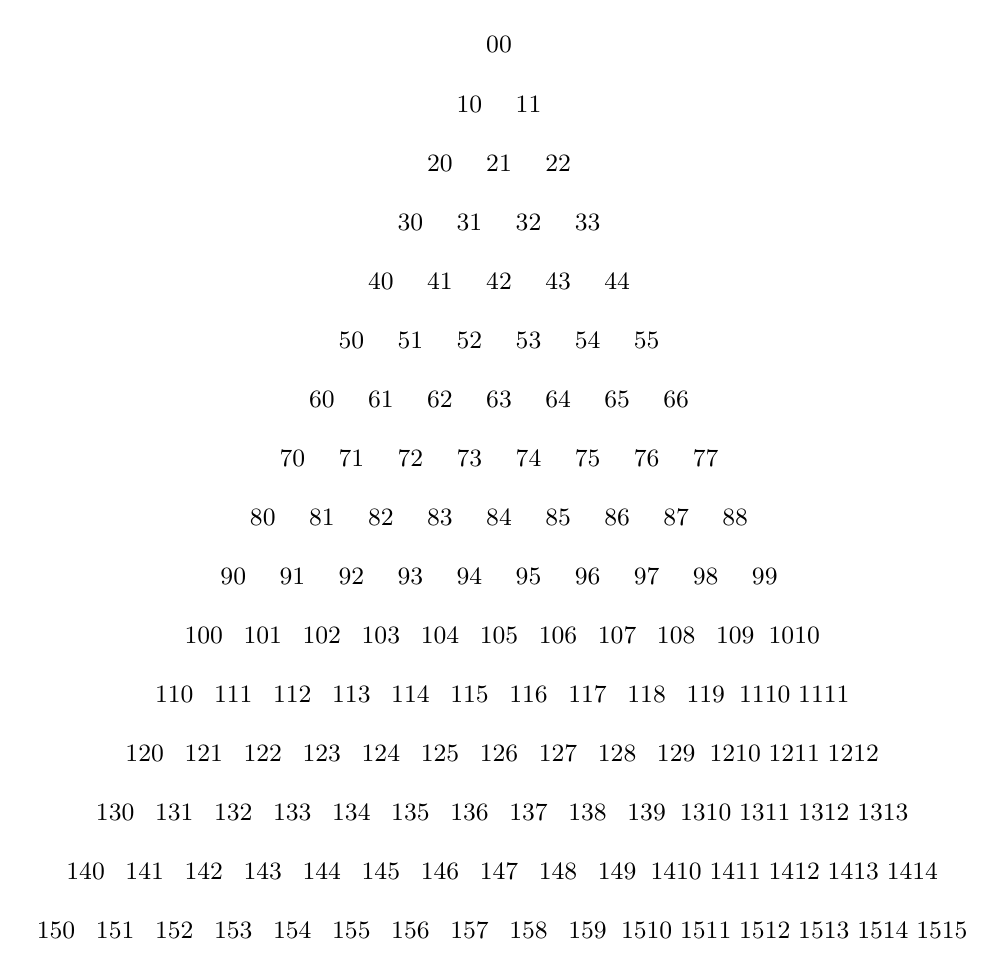
\begin{tikzpicture}[scale=.75]
\foreach \n in {0,...,15} {
  \foreach \k in {0,...,\n} {
    \node at (\k-\n/2,-\n) {\small{\(\binomialCoefficient{\n}{\k}\)}};
  }
}
\end{tikzpicture}
\end{document}
\end{center}
\end{problem}
\begin{answer}{induction:pascal}
When we expand out \((1+x)^n\), each term in the expansion arises from choosing either \(1\) or \(x\) from each factor \(1+x\), and multiplying out the choices to produce the term.
So terms with \(x^k\) arise when we choose \(x\) from \(k\) of the factors \(1+x\), and \(1\) from the other \(n-k\).
So in \((1+x)^{n+1}\), the \(x^k\) terms arise from choosing \(x\) from \(k\) of the first \(n\) factors \(1+x\), and choosing \(1\) from the last one, or from choosing \(x\) from \(k-1\) of the first \(n\) factors, and also choosing \(x\) from the last one.
\end{answer}
\begin{problem}{induction:cyclotomic}
For each positive integer \(n\), let
\[
p_n(x)\defeq 1+x+\dots+x^{n-1}=\sum_{k=0}^{n-1} x^k.
\]
Prove that
\[
p_n(1+x)=\sum_{k=0}^{n-1} \binom{n}{k+1}x^k.
\]
\end{problem}
\begin{answer}{induction:cyclotomic}
For \(n=1,2,3\), we can check by hand:
\[
\begin{array}{ccc}
\toprule
n & p_n(x) & p_n(1+x) \\
\midrule
1 & 1 & 1 \\
2 & 1+x & 2+x=\binom{2}{1}x^0+\binom{2}{2}x^1\\
3 & 1+x+x^2 & 3+3x+x^2=\binom{3}{1}x^0+\binom{3}{2}x^1+\binom{3}{3}x^2 \\
\bottomrule
\end{array}
\]
From then on, we will need to use induction: 
\[
p_{n+1}(x)=p_n(x)+x^n,
\]
so
\begin{align*}
p_{n+1}(1+x)
&=
p_n(1+x)+(1+x)^n
\\
&=
\sum_{k=0}^{n-1} \binom{n}{k+1}x^k
+
\sum_{k=0}^n \binom{n}{k}x^k,
\\
&=
\sum_{k=0}^{n-1} \left( \binom{n}{k+1}+\binom{n}{k}\right)x^k+x^n,
\\
&=
\sum_{k=0}^{n-1} \binom{n+1}{k+1}x^k+x^n,
\\
&=
\sum_{k=0}^n\binom{n+1}{k+1}x^k.
\end{align*}
\end{answer}

\section{Sage}
\epigraph[author={Emo Philips}]{A computer once beat me at chess, but it was no match for me at kick boxing.}\SubIndex{Philips, Emo}\SubIndex{kick boxing}
To define a function in sage, you type \texttt{def}, to mean \emph{define}, like:
\begin{sageblock}
def f(n):
    return 2*n+1
\end{sageblock}
and press \emph{shift--enter}.
For any input \(n\), it will return a value \(f(n)=2n+1\). 
Careful about the \verb!*! for multiplication.  
Use your function, for example, by typing
\begin{sageblock}
f(3)
\end{sageblock}
and press \emph{shift--enter} to get \(\sage{f(3)}\).

A function can depend on several inputs:
\begin{sageblock}
def g(x,y):
    return x*y+2
\end{sageblock}
A \emph{recursive function}\define{function!recursive}\define{recursive function} is one whose value for some input depends on its value for other inputs.
For example, the sum of the integers from \(1\) to \(n\) is:
\begin{sageblock}
def sum_of_integers(n):
    if n<=0: 
        return 0
    else: 
        return n+sum_of_integers(n-1)
\end{sageblock}
giving us \verb!sum_of_integers(5)!\({}=\sage{sum_of_integers(5)}\).
\begin{problem}{induction:fibonacci}
The \emph{Fibonnaci sequence}\SubIndex{Fibonacci sequence} is \(F(1)=1\), \(F(2)=1\), and \(F(n)=F(n-1)+F(n-2)\) for \(n \ge 3\).
Write out a function \texttt{F(n)} in sage to compute the Fibonacci sequence.
\end{problem}
%\begin{answer}{induction:fibonacci}
%\begin{sageblock}
%def F(n):
%    if n==0: return 0
%    elif n==1: return 1
%    else: return F(n-1)+F(n-2)
%\end{sageblock}
%\end{answer}
Lets check that \(2^{n+1} < 3^n\) for some values of \(n\), using a loop:
\begin{sageblock}
for n in [0..10]: 
    print(n,3^n-2^(n+1))
\end{sageblock}
This will try successively plugging in each value of $n$ starting at $n=0$ and going up to $n=1$, $n=2$, and so on up to $n=10$, and print out the value of $n$ and the value of $3^n-2^{n+1}$.
It prints out:
\begin{verbatim}
(0, -1)
(1, -1)
(2, 1)
(3, 11)
(4, 49)
(5, 179)
(6, 601)
(7, 1931)
(8, 6049)
(9, 18659)
(10, 57001)
\end{verbatim}
giving the value of $n$ and the value of the difference $3^n-2^{n+1}$, which we can readily see is positive once $n \ge 2$.
Tricks like this help us to check our induction proofs.

If we write \verb!a=a+1! in sage, this means that the new value of the variable \verb!a! is equal to one more than the old value that \verb!a! had previously.
Unlike mathematical variables, sage variables can change value over time.
In sage the expression \verb!a!=b! means \(a \ne b\).
Although sage knows how to calculate the greatest common divisor of some integers, we can define own greatest common divisor function:
\begin{sageblock}
def my_gcd(a, b):
    if abs(a)<abs(b):
        b,a=a,b
    while b!=0:
        a,b=b,a%b 
    return abs(a)
\end{sageblock}
We could also write a greatest divisor function that uses repeated subtraction, avoiding the quotient operation {\%}:
\begin{sageblock}
def gcd_by_subtraction(a, b):
    if a<0:
        a=-a
    if b<0:
        b=-b
    if a==0:
        return b
    if b==0:
        return a    
    while a!=b:
        if a>b:
            a=a-b
        else:
            b=b-a
    return a
\end{sageblock}

\section{Lists in sage}
Sage manipulates lists.\define{list} 
A list is a finite sequence of objects written down next to one another.
The list \verb!L=[4,4,7,9]! is a list called \(L\) which consists of four numbers: \(4, 4, 7\) and \(9\), in that order.
Note that the same entry can appear any number of times; in this example, the number \(4\) appears twice.
You can think of a list as like a vector in \(\R{n}\), a list of numbers.
When you ``add'' lists they concatenate: \verb![6]+[2]! yields \(\sage{[6]+[2]}\).
Sage uses notation \verb!L[0]!, \verb!L[1]!, and so on, to retrieve the elements of a list, instead of the usual vector notation.
\emph{Warning:} the element \verb!L[1]! is \emph{not} the first element.
The length of a list \(L\) is \verb!len(L)!.
To create a list \([0,1,2,3,4,5]\) of successive integer, type \verb!list(range(0,6))!.
Note that the number 6 here tells you to go up to, but not include, 6.
So a \(L\) list of \(6\) elements has elements \(L_0, L_1, \dots, L_5\), denoted \verb!L[0]!, \verb!L[1]!, \dots, \verb!L[5]! in sage.
To retrieve the list of elements of \(L\) from \(L_2\) to \(L_4\), type \verb!L[2:5]!; again strangely this means up to but not including \(L_5\).

We create a list with 10 entries, print it:
\begin{sageblock}
L=list(range(0,10))
print(L)
\end{sageblock}
yielding \(\sage{L}\) and then print its reversal:
\begin{sageblock}
print(L.reverse())
\end{sageblock}
yielding \(\sage{L.reverse()}\).

We can construct a list of elements of the Fibonacci\SubIndex{Fibonacci sequence} sequence:
\begin{sageblock}
def fibonacci_list(n):
    L=[1,1]
    for i in range(2,n):
        L=L+[L[i-1]+L[i-2]]
    return L
\end{sageblock}
so that \verb!fibonacci_list(10)! yields \(\sage{fibonacci_list(10)}\), a list of the first ten numbers in the Fibonacci sequence.
The code works by first creating a list \verb!L=[1,1]! with the first two entries in it, and then successively building up the list \(L\) by concatenating to it a list with one more element, the sum of the two previous list entries, for all values \(i=2,3,\dots,n\).

